This is the Open\-C\-L version of J\-T\-C extra stuff \hypertarget{index_Introduction}{}\section{Introduction}\label{index_Introduction}
The rapid development of parallel hardware in the last decade requires a constant evaluation of the parallel algoritms used in large scale scientific applications . Iterative kernels are essential components of iterative solvers which are the preferred technique in a variety of large scale problems. Jacobi iteration for the second order discretisation of the Laplacian $ 3D$ operator\-: \begin{equation} u^{(new)}_{i,j,k}=\frac{1}{6}(u^{(old)}_{i-1,j,k}+ u^{(old)}_{i+1,j,k}+u^{(old)}_{i,j-1,k}+ u^{(old)}_{i,j+1,k}+u^{(old)}_{i,j,k-1}+u^{(old)}_{i,j,k+1}) \ , \end{equation} is the one of the simplest, yet not trivial, example of iterative kernel. In its simple form it contains the features relevant to the performance for a large class of iterators\-: i) stranded memory access and ii) low number of floating point operations per memory reference. \hypertarget{index_Results}{}\section{Results}\label{index_Results}

\begin{DoxyImage}
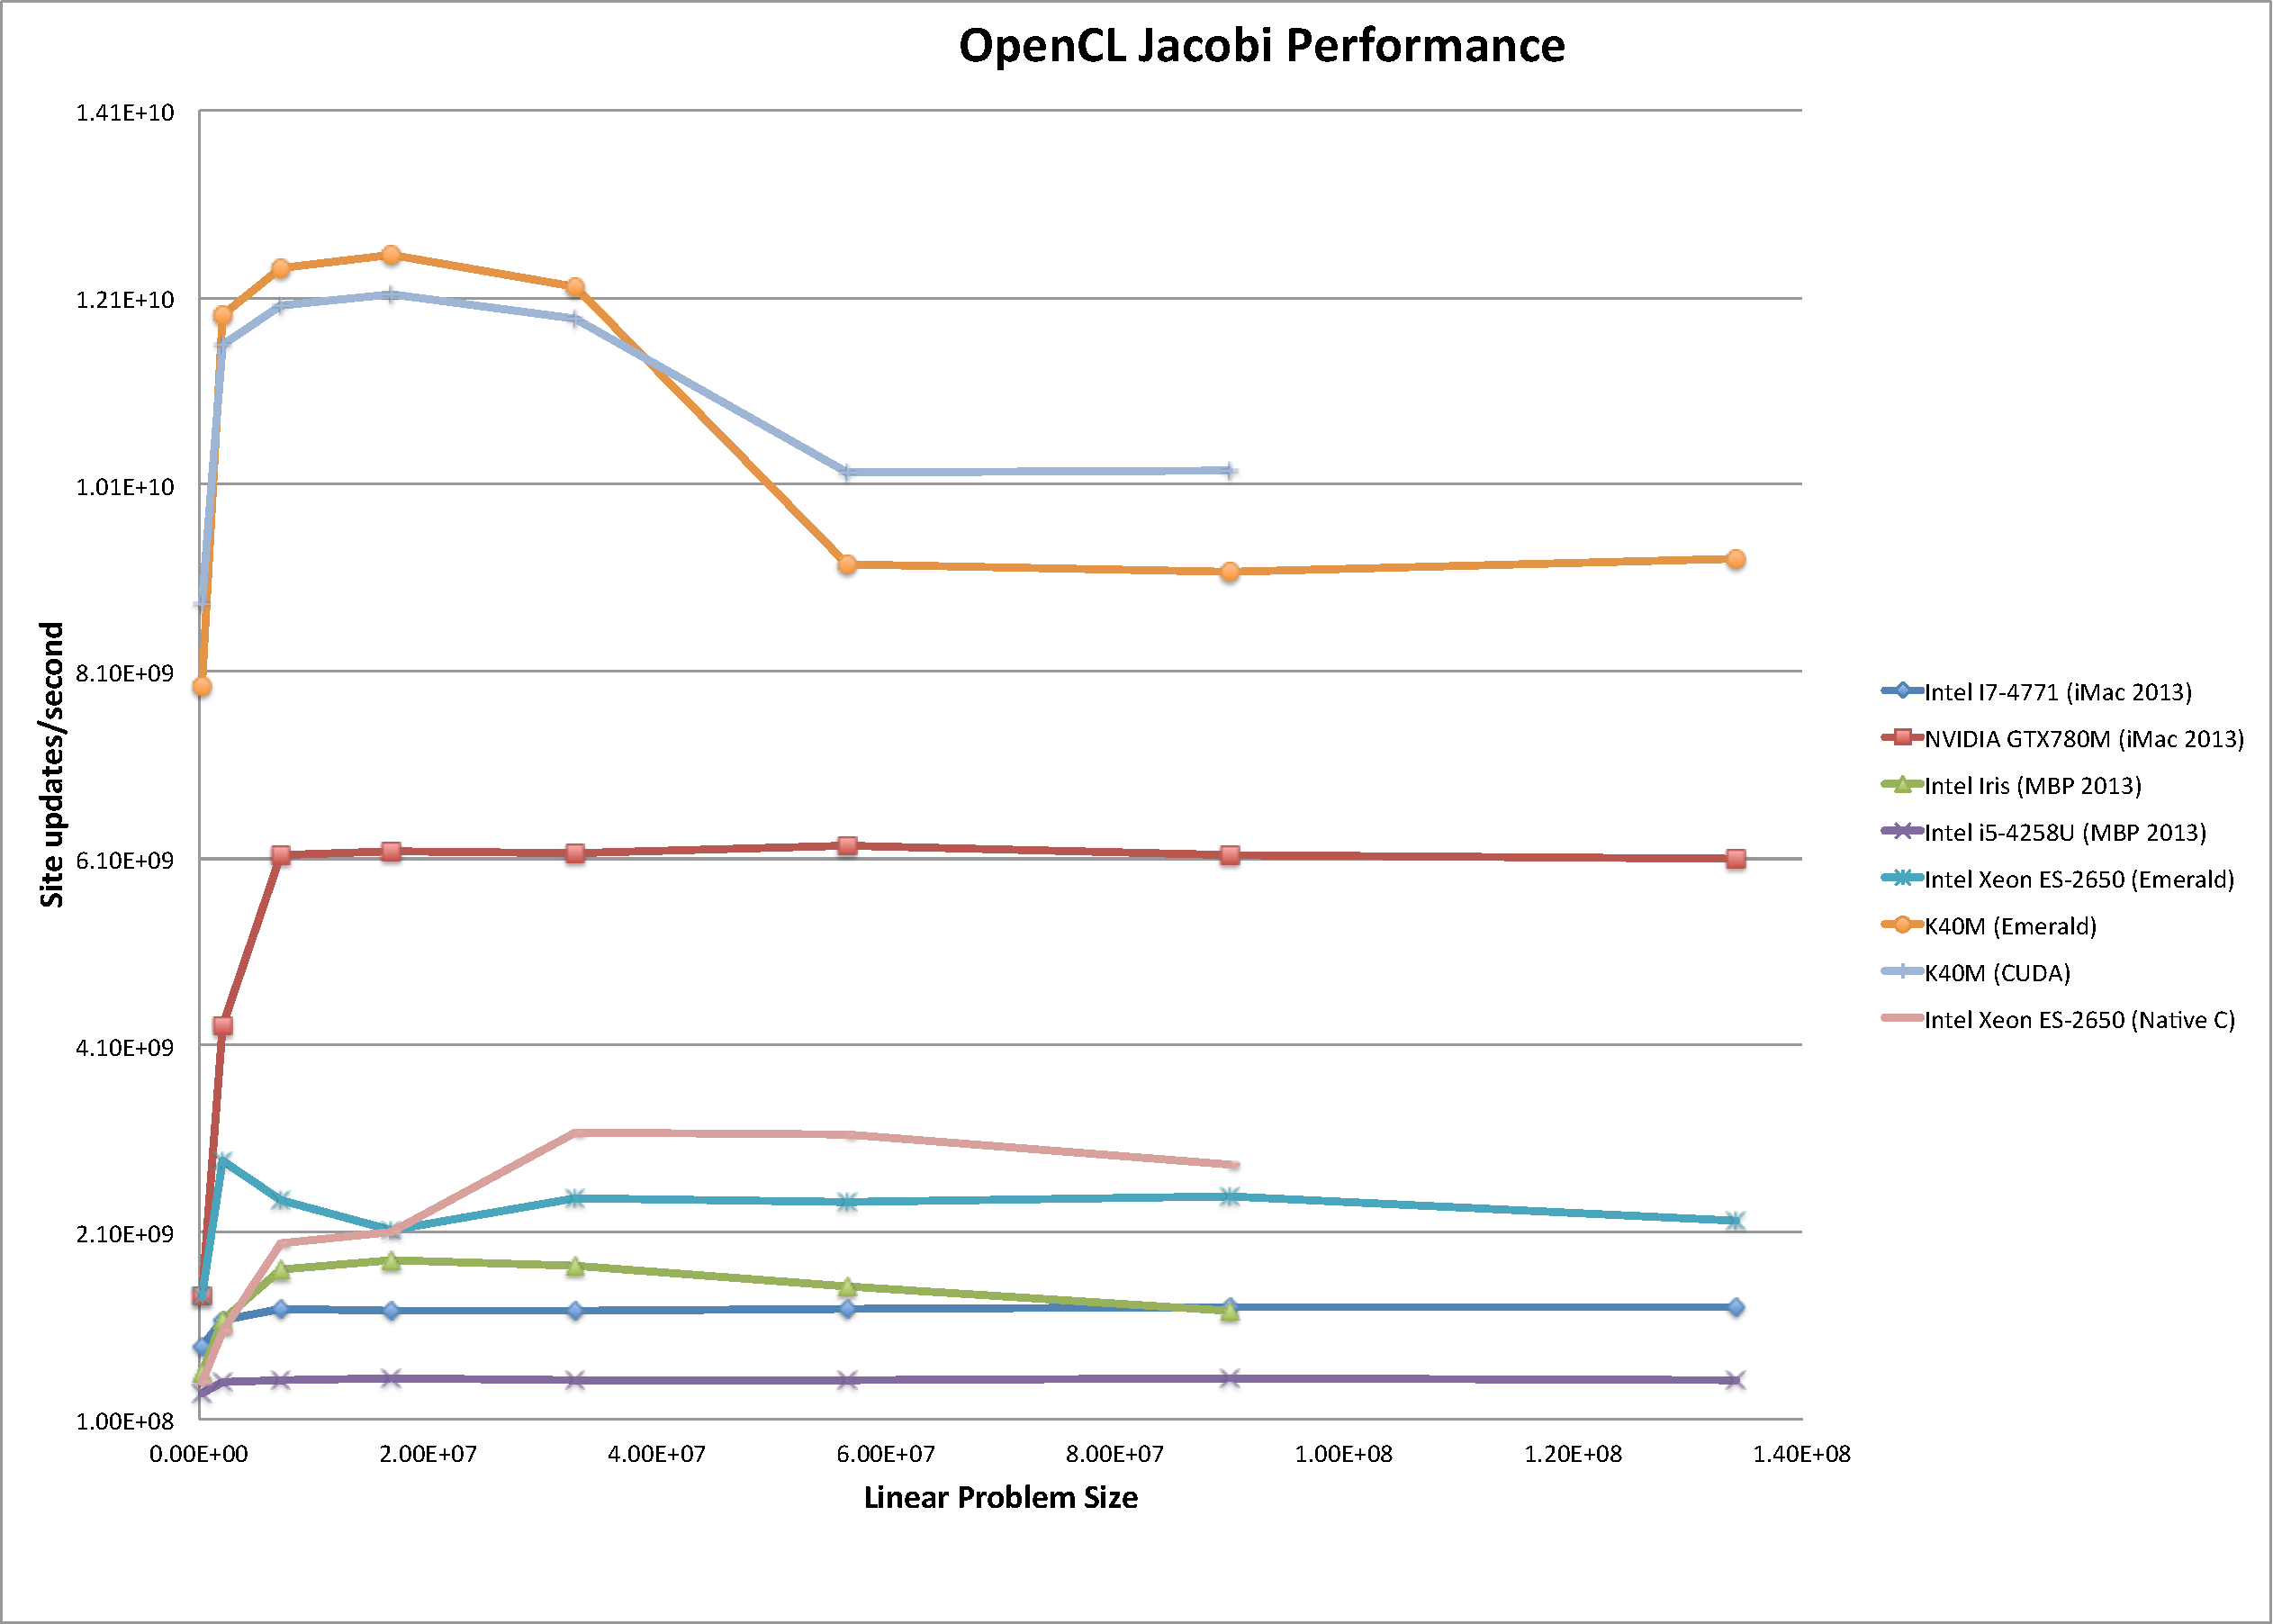
\includegraphics[width=10cm]{OPENCLRESULTS}
\caption{My application}
\end{DoxyImage}
 